% !TEX root = ../CINTA-cn.tex
%%%%%%%%%%%%%%%%%%%%%%%%%%%%%%%%%%%%%%%%%%%%%%%%%%%%%%%%%%%%%%%%%%%%
% Author: Libin Wang
% Appendix 
% This document was released as open source on 2026-06-18.
% Copyright 2023, Libin Wang. Creative Commons License
% This work is licensed under a Creative Commons Attribution-NonCommercial-NoDerivatives 4.0 International License.

%%%%%%%%%%%%%%%%%%%%%%%%%%%%%%%%%%%%%%%%%%%%%%%%%%%%%%%%%%%%%%%%%%%
\appendix

\chapter{快速乘法算法}
\label{chap:fast_mul}

设$a$和$b$是两个$n$比特整数，为了方便，也与实际应用相符，假定$n = 2^k$，$k$是某个正整数。
 该算法使用
 \textit{分治法}\index{分治法}
（\textit{divide-and-conquer}）\index{divide-and-conquer}为策略计算$ab$。
首先，分别把$a$和$b$写为两部分，每部分$n/2$比特：
\[ a = 2^{n/2}a_L + a_R\]
\[b = 2^{n/2} b_L + b_R\]

那么，$a$与$b$的乘积可写为：
\[ ab =(2^{n/2}a_L + a_R)(2^{n/2} b_L + b_R) = 2^n a_L b_L + 2^{n/2}(a_L b_R + a_R b_L) + a_R b_R.\]
使用等式最右边的表达计算$ab$，正确性是显然的。

为了分析算法的效率，先得到算法开销的递归式如下：
\[T(n) = 3T(n/2) + \mathcal{O}(n)\]
即表示存在一个常数$C$使得
\begin{equation}
\label{eq:A01}
T(n) \leq 3T(n/2) + Cn
\end{equation}

以下我们要证明：
\begin{equation}
\label{eq:A02}
T(2^n) = c(3^n - 2^n),
\end{equation}
其中，$c$是$T(2)$和$C$（这是等式~\ref{eq:A01}中的常量）中的最大值。


\begin{proof}
使用数学归纳法证明。

归纳初始. 当$k = 1$，有$T(2) \leq c(3^1 - 2^1) = c$，因为$c$是$T(2)$和$C$中的最大值。

归纳假设. 假设 
\[T(2^k) \leq c(3^k - 2^k)\]

归纳步. 根据等式~\ref{eq:A01}，有：
\begin{align*}
T(2^{k+1}) &\leq 3T(2^k) +C2^k\\
                    &\leq 3c(3^k - 2^k) + C2^k\\
                    &\leq c3^{k+1} - c\cdot 3\cdot 2^k + c2^k\\
                    &\leq c(3^{k+1} - 2^{k+1}).
\end{align*} \qed
\end{proof}

\begin{theorem}{}{fast_mul}
	两个$n$比特整数的乘法的计算开销是$\mathcal{O}(n^{\log_2\; 3})$比特运算。（注意：$\log_2 \; 3$ 约等于$1.585$。）
\end{theorem}

\begin{proof}
根据等式~\ref{eq:A02}得到：
	\begin{align*}
	T(n) &= T(2^{\log_2\; n}) \leq T(2^{\lfloor \log_2 \; n\rfloor + 1})\\
	         &\leq c(3^{\lfloor \log_2 \; n \rfloor+ 1} - 2^{\lfloor \log_2 \; n \rfloor+ 1})\\
	         &\leq3c\cdot 3^{\lfloor \log_2 \; n \rfloor} \leq 3c\cdot 3^{\log_2 \; n }\\
	         &= 3cn^{\log_2\; 3} .
	\end{align*}
	因为$3^{\log_2 \; n} = n^{\log_2 \; 3}$，最后那个等号成立。
	所以，$T(n)=\mathcal{O}(n^{\log_2\; 3})$。
\end{proof}

\chapter{斐波那契数列}
\label{chap:fib}

\begin{align*}
F_0 &= 0\\
F_1 &= 1 \\
F_n &= F_{n-1} + F_{n-2}.
\end{align*}

\begin{center}
	\lstinputlisting[caption = "Fibonacci Number."]{codes/appendix-1.py}
\end{center}

\begin{center}
	\lstinputlisting[caption = "Measure the ratio."]{codes/appendix-2.py}
\end{center}

\begin{align*}
	F_3 / F_2 &= 2.000000000  \qquad F_4 / F_3 = 1.500000000\\
    F_5 / F_4 &= 1.666666667  \qquad F_6 / F_5 = 1.600000000\\
    F_7 / F_6 &= 1.625000000  \qquad F_8 / F_7 = 1.615384615\\
    F_9 / F_8 &= 1.619047619  \qquad F_{10} / F_9 = 1.617647059\\
    F_{11} / F_{10} &= 1.618181818  \qquad  F_{12} / F_{11} = 1.617977528\\
    F_{13} / F_{12} &= 1.618055556  \qquad F_{14} / F_{13} = 1.618025751\\
    F_{15} / F_{14} &= 1.618037135   \qquad F_{16} / F_{15} = 1.618032787
\end{align*}

\[F_n \approx \alpha F_{n-1}\]

\chapter{生日悖论}
\label{chap:birthday}
所谓\emph{生日悖论}问题即：问在$n$个人当中，有两个或以上的人生日相同的概率为多少？准确来说，这不是\emph{悖论}，
只是稍微违反人类直觉罢了。结论是，如果$n=23$，则有两个人生日相同的概率超过$50\%$。这个结论是假定每个人的生日都是
从一年$365$天这个范围内均匀随机选取的日子。$n=23$这个答案是否出乎你的预料呢？以下讨论这个概率如何得到。

假设我们有一个盒子里面放了$m$个球，每一球都用标签唯一标注一个号码，范围从$1$到$m$。然后抽取$k$个球，如抽彩票一般，抽完了
球还放回去。问以下问题：抽取到同一个球的概率有多大？抽取到同一个球这个事件也称发生了一次碰撞。

注意到，抽取第二个球不与第一个球相同的概率是$1 - 1/m$，而第三个球不与前面抽到的球相同的概率是$1 - 2/m$。
以这种方式思考，得到：
\begin{equation}
\label{eq:A03}
\Pr(\text{不发生碰撞}) = \prod_{i=0}^{k-1} (1 - i/m)
\end{equation}
如果$k \le m$，则可以把$1-i/m$换为$e^{-i/m}$，然后公式~\ref{eq:A03}可以重写为：

\begin{align*}
\Pr(\text{不发生碰撞}) &= \prod_{i=0}^{k-1} (1 - i/m)\\
                                 &\thickapprox \prod_{i=0}^{k-1} e^{-i/m} \\
                                 &= e^{- \sum_{i=0}^{k-1} (i/m)}\\
                                 &= e^{-k(k-1)/2m} \\
                                 &\thickapprox e^{-k^2/2m}.                             
\end{align*}

\begin{align}
\Pr(\text{发生碰撞}) &= 1 - \Pr(\text{不发生碰撞})\\
                         &= 1 - e^{-k^2/2m}
\end{align}

希望以$50\%$的概率发生一次碰撞，则$k = \sqrt{2\ln\;2m} \thickapprox 1.18\sqrt{m}$。原始的生日悖论问题中$m = 365$，
则得到$k = \sqrt{(2 \ln\; 2) \cdot 365} \thickapprox 23$。
下图展示了$m = 365$，$k$取不同值时发生碰撞的概率，可知当$k = 50$时概率基本为$1$。也就是说一个$50$人的班级大概率有两位同学会同一天过生日。

\begin{figure}
	\begin{center}
		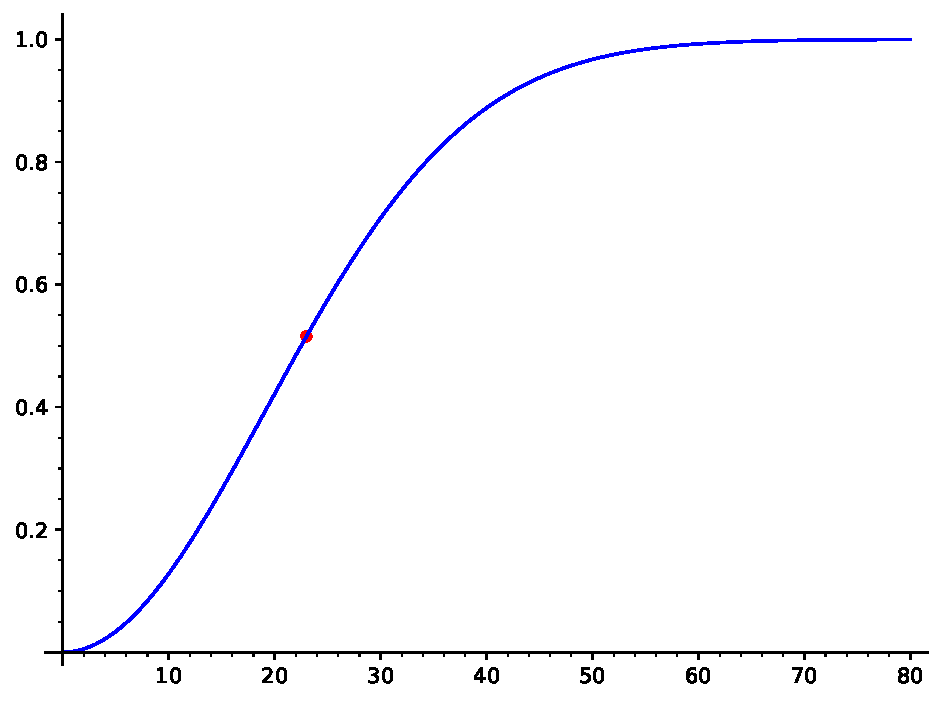
\includegraphics[width=0.5\textwidth]{figures/chapt99-1-birthday-collision-probability.pdf}
		\caption{生日悖论问题的概率.}
	\end{center}
	\label{fig:birth}       % Give a unique label
\end{figure}

\chapter{数论中的“一”}
\label{chap:one}
以下列举若干数论中出现的“1”（或$-1$），即与$1$相关的公式。

\begin{enumerate}
\item $(-1)^2 = 1$

\item $ (n-1)^2 \equiv 1 \pmod{n}$，对任意的整数$n$，$n-1$是模$n$下的$-1$。

\item 对任意互素的整数$a$和$b$，存在整数$s$和$t$使得：$as + bt = 1$。

\item 对任意互素的整数$a$和$b$，$\gcd(a, b) =1$。

\item $a a^{-1} \equiv 1 \pmod{n}$，即$a$与$a^{-1}$在模$n$下互为乘法逆元。

\item 威尔逊定理：$(p-1)! \equiv - 1 \pmod{p}$，$p$为素数。

\item 费尔马小定理：$a^{p-1} \equiv 1 \pmod{p}$，$p$为素数，$a$与$p$互素。

\item 欧拉定理：$a^{\phi(n)} \equiv 1 \pmod{n}$，$a$与$n$互素。

\item 群论费尔马小定理：对任意$n$阶有限群$\mathbb{G}$，记$1$是群的单位元。任取元素$a\in \mathbb{G}$，有$a^n = 1$。

\item 勒让德符号：$\left(\frac{a}{p}\right) = 1$，若$a$是模$p$的二次剩余，$p$为素数，$a$与$p$互素。

\item  欧拉公式：$e^{i \pi} =  -1$。
\end{enumerate}
